%-------------------------------------------------------------------------------

% This file is part of Code_Saturne, a general-purpose CFD tool.
%
% Copyright (C) 1998-2014 EDF S.A.
%
% This program is free software; you can redistribute it and/or modify it under
% the terms of the GNU General Public License as published by the Free Software
% Foundation; either version 2 of the License, or (at your option) any later
% version.
%
% This program is distributed in the hope that it will be useful, but WITHOUT
% ANY WARRANTY; without even the implied warranty of MERCHANTABILITY or FITNESS
% FOR A PARTICULAR PURPOSE.  See the GNU General Public License for more
% details.
%
% You should have received a copy of the GNU General Public License along with
% this program; if not, write to the Free Software Foundation, Inc., 51 Franklin
% Street, Fifth Floor, Boston, MA 02110-1301, USA.

%-------------------------------------------------------------------------------

\programme{covofi}\label{ap:covofi}
%
\vspace{1cm}
%-------------------------------------------------------------------------------
\section*{Fonction}
%-------------------------------------------------------------------------------
Dans ce sous-programme, on r\'{e}sout : \\
{\tiny$\bigstar$} soit l'\'{e}quation de convection-diffusion d'un scalaire en
pr\'{e}sence de termes sources :
%\begin{equation}\label{Base_Covofi_EQ_cvd)
\begin{equation}
\frac {\partial  (\rho a)}{\partial t} +
\underbrace{\,\dive\,((\rho \underline{u})\,a)}_{\text{convection}}
- \underbrace{\,\dive\,(K \grad a)}_{\text{diffusion}} = T_s^{\,imp} a
+T_s^{\,exp} +\Gamma\,a_i
\end{equation}
Ici $a$ repr\'{e}sente la valeur instantan\'{e}e du scalaire en approche laminaire ou,
en approche RANS, sa moyenne de Reynolds $\widetilde{a}$. Les deux approches
\'{e}tant exclusives et les \'{e}quations obtenues similaires, on utilisera le plus
souvent aussi la notation $a$ pour $\widetilde{a}$.\\
{\tiny$\bigstar$} soit, dans le cas d'une mod\'{e}lisation RANS, la variance de la
fluctuation d'un scalaire en pr\'{e}sence de termes sources\footnote{Davroux A. et
Archambeau F. : Calcul de la variance des fluctuations
d'un scalaire dans le solveur commun. Application \`{a} l'exp\'{e}rience du CEGB dite
``Jet in Pool'', HE-41/99/043.} :
\begin{equation}
\begin{array}{lcl}
&\displaystyle
 \frac {\partial  (\rho \widetilde{{a"}^2})}{\partial t} +
\underbrace{\dive\,((\rho\,\underline{u})\ \widetilde{{a"}^2})}_{\text{convection}}
- \underbrace{\dive\,(K\ \grad \widetilde{{a"}^2})}_{\text{diffusion}} = T_s^{\,imp} \widetilde{{a"}^2}
+T_s^{\,exp} +\ \Gamma\,\widetilde{{a"}^2}_i \\
&\displaystyle \underbrace {+ 2\,\frac{\mu_t}{\sigma_t}(\grad \widetilde{a})^2 -
\frac{\rho\,\varepsilon}{R_f k}\ \widetilde{{a"}^2}}_{\text{termes de production et
de dissipation dus \`{a} la turbulence moyenne}}
\end{array}
\end{equation}
$\widetilde{{a"}^2}$ repr\'esente ici la moyenne du carr\'e des fluctuations\footnote{$a$ et
$\widetilde{{a"}^2}$, sous forme discr\`ete en espace, correspondent donc en
fait \`a des vecteurs dimensionn\'es \`a \var{NCELET} de composantes $a_I$ et $\widetilde{{a"}^2}_{I}$
respectivement, I d\'ecrivant l'ensemble des cellules.} de $a$. $K$, $\Gamma$,
$T_s^{imp}$ et  $T_s^{exp}$ repr\'{e}sentent respectivement le coefficient de
diffusion, la valeur du terme source de masse, les termes sources implicite et
explicite du scalaire $a$ ou $\widetilde{{a"}^2}$. $\mu_t$ et $\sigma_t$
sont respectivement la viscosit\'{e} turbulente et le nombre de Schmidt ou de
Prandtl turbulent, $\varepsilon$ est la dissipation de l'\'{e}nergie turbulente $k$
et $R_f$ d\'{e}finit le rapport constant entre les \'{e}chelles dissipatives de $k$ et
de $\widetilde{{a"}^2}$ ($R_f$ est constant selon le mod\`{e}le assez simple adopt\'{e} ici).\\
On \'{e}crit les deux \'{e}quations pr\'{e}c\'{e}dentes sous la forme commune suivante~:
\begin{equation}
\frac {\partial  (\rho f)}{\partial t} + \dive\,((\rho\,\underline{u}) f)
- \dive\,(K \grad f) = T_s^{\,imp} f + T_s^{\,exp} + \Gamma\,f_i + T_s^{\,pd}
\end{equation}
avec, pour $f=a$ ou $f=\widetilde{{a"}^2}$ :\\
\begin{equation}
\begin{array}{lll}
&\displaystyle
T_s^{\,pd}=
\begin{cases}
0 & \text{pour $f=a$}, \\
2\ \displaystyle \frac{\mu_t}{\sigma_t}(\grad \widetilde{a})^2 -
\displaystyle \frac{\rho\,\varepsilon}{R_f k}\ \widetilde{{a"}^2} & \text{pour $f=\widetilde{{a"}^2}$ }
\end{cases}
\end{array}
\end{equation}

Le terme $\displaystyle \frac {\partial  (\rho f)}{\partial t}$ est d\'{e}compos\'{e} de la sorte :
\begin{equation}
\frac {\partial  (\rho f)}{\partial t}=\rho \frac {\partial f}{\partial t} + f
\frac {\partial \rho}{\partial t}
\end{equation}
En utilisant l'\'{e}quation de conservation de la masse (cf. \fort{predvv}),
l'\'{e}quation pr\'{e}c\'{e}dente s'\'{e}crit finalement :\\
\begin{equation}\label{Base_Covofi_Eq_cv_scal}
\rho\ \displaystyle \frac {\partial f}{\partial t} +
\dive\,((\rho\,\underline{u})\,f) - \dive\,(K\ \grad f)
= T_s^{\,imp} f + T_s^{\,exp} + \Gamma (f_i - f) + T_s^{\,pd} + f\,\dive\,(\rho\,\underline{u})
\end{equation}

%%%%%%%%%%%%%%%%%%%%%%%%%%%%%%%%%
%%%%%%%%%%%%%%%%%%%%%%%%%%%%%%%%%%
\section*{Discr\'etisation}
%%%%%%%%%%%%%%%%%%%%%%%%%%%%%%%%%%
%%%%%%%%%%%%%%%%%%%%%%%%%%%%%%%%%%
Pour int\'{e}grer l'\'{e}quation (\ref{Base_Covofi_Eq_cv_scal}), une discr\'{e}tisation temporelle de
type $\theta$-sch\'{e}ma est appliqu\'{e}e \`{a} la variable r\'{e}solue\footnote{Si
$\theta=1/2$, ou qu'une extrapolation est utilis\'{e}e, le pas de temps $\Delta t$
est suppos\'{e} uniforme en temps et en espace.}~:
\begin{equation}
f^{n+\theta} = \theta \,\, f^{n+1} + (1-\theta)\,\, f^{n}
\end{equation}

L'\'{e}quation (\ref{Base_Covofi_Eq_cv_scal}) est discr\'etis\'ee au temps $n+\theta$ en
supposant les termes sources explicites pris au temps $n+\theta_{S}$, et ceux
implicites en $n+\theta$.
Par souci de clart\'{e}, on suppose, en l'absence d'indication, que les propri\'{e}tes
physiques $\Phi$ ($K,\,\rho$,...) et le flux de masse $(\rho\,\underline{u})$
sont pris respectivement aux instants $n+\theta_\Phi$ et $n+\theta_F$, o\`{u}
$\theta_\Phi$ et $\theta_F$ d\'{e}pendent des sch\'{e}mas en temps sp\'{e}cifiquement
utilis\'{e}s pour ces grandeurs\footnote{cf. \fort{introd}}.

\begin{equation}
\begin{array}{lcl}
&\displaystyle
 \rho \frac {f^{n+1}-f^{n}}{\Delta t} +
\underbrace{\dive\,((\rho\,\underline{u})\,f^{n+\theta})}_{\text{convection}}
- \underbrace{\dive\,(\,K\,\grad f^{n+\theta})}_{\text{diffusion}} =
T_s^{\,imp}\,f^{n+\theta} + T_s^{\,exp,\,n+\theta_{S}}\\
& + (\Gamma\,f_i)^{n+\theta_{S}}-\Gamma^{n}\,f^{n+\theta} +\
T_s^{\,pd,\,n+\theta_S} + f^{n+\theta}\,\dive\,(\rho\underline{u})
\end{array}
\end{equation}
o\`{u} :
\begin{equation}
 T_s^{\,pd,\,n+\theta_S} =
\begin{cases}
0 & \text{pour $f=a$}, \\
2 \displaystyle \left[\frac{\mu_t}{\sigma_t}(\grad \widetilde{a})^2\right]^{n+\theta_S}-\frac{\rho\,
\varepsilon^{n}}{R_f\,k^{n}}(\widetilde{{a"}^2})^{n+\theta}& \text{pour $f=\widetilde{{a"}^2}$ }
\end{cases}
\end{equation}
Le terme de production affect\'{e} d'un indice $n+\theta_{S}$ est un terme source
explicite et il est donc trait\'{e} comme tel :
\begin{equation}
\begin{array}{rll}
\displaystyle
\left[\frac{\mu_t}{\sigma_t}(\grad
\widetilde{a})^2\right]^{n+\theta_{S}}&=&\displaystyle
(1+\theta_{S})\,\,\frac{\mu_t^{n}}{\sigma_t}(\grad
\widetilde{a}^{n})^2-\theta_{S}\,\,\frac{\mu_t^{n-1}}{\sigma_t}(\grad
\widetilde{a}^{n-1})^2\\
\end{array}
\end{equation}
\\

L'\'{e}quation (\ref{Base_Covofi_Eq_cv_scal}) s'\'ecrit :
\begin{equation}\label{Base_Covofi_Eq_scal_tempo}
\begin{array}{c}
\displaystyle
 \rho\,\frac {f^{n+1}-f^{n}}{\Delta t} +
\theta \,\,\dive\,((\rho\,\underline{u})\,f^{n+1})- \theta \,\,\dive\,(\,K\ \grad f^{n+1})
\\
-\left[ \theta\,\, T_s^{\,imp}\,- \theta\,\, \Gamma^{n} + \theta\,\, T_s^{\,pd,\,imp}+\theta\,\,
\dive\,(\rho\ \underline{u})\right]\,f^{n+1}
\\
= (1-\theta)\,\,T_s^{\,imp}\,f^{n} + T_s^{\,exp,\,n+\theta_S} +
(\Gamma\,f_i)^{n+\theta_S}-(1-\theta)\,\,\Gamma^{n}\,
f^{n}+ T_s^{\,pd,\,exp}-\theta\,T_s^{\,pd,\,imp}\,f^{n}
\\
+ (1-\theta) \,\, f^{n}\,\dive\,(\rho\ \underline{u})- (1-\theta) \,\, \dive\,((\rho\,\underline{u})\,f^{n})
+ (1-\theta)\,\, \dive\,(\,K\ \grad f^{n})
\end{array}
\end{equation}
avec :
\begin{equation}
T_s^{\,pd,\,imp} =
\begin{cases}
0 & \text{pour $f=a$}, \\
- \displaystyle \frac{\rho\,\varepsilon^n}{R_f \,k^n} &  \text{pour $f=\widetilde{{a"}^2}$}
\end{cases}
\end{equation}
\begin{equation}
T_s^{\,pd,\,exp}=
\begin{cases}
0 & \text{pour $f=a$}, \\
2\ \displaystyle\left[\frac{\mu_t}{\sigma_t}(\grad
\widetilde{a})^2\right]^{n+\theta_S} -
\frac{\rho\,\varepsilon^n}{R_f\,k^n}(\widetilde{{a"}^2})^n & \text{pour
$f=\widetilde{{a"}^2}$}
\end{cases}
\end{equation}
On rappelle que, pour un scalaire $f$, le sous-programme \fort{codits}
r\'{e}sout une \'{e}quation du type suivant
\label{Base_Covofi_Eq_Codits}
\begin{equation}
\begin{array}{c}
\displaystyle f_s^{\,imp} (f^{n+1} - f^{n}) +
\theta \,\, \dive((\rho\,\underline{u})\,f^{n+1})- \theta \,\, \dive\,(\,K\,\grad f^{n+1})
\\
= f_s^{\,exp} -\underbrace{(1-\theta) \,\, \dive((\rho\,\underline{u})\,f^{n}) + (1-\theta)
\,\, \dive\,(\,K\,\grad f^{n})}_{\text{convection diffusion explicite}}
\end{array}
\end{equation}
$f_s^{exp}$ repr\'{e}sente les termes sources discr\'etis\'es de mani\`ere explicite
en temps (hormis contributions de la convection diffusion explicite provenant du
$\theta$-sch\'ema) et $f_s^{imp}\,f^{n+1}$ repr\'esente les termes lin\'eaires
en $f^{n+1}$ dans l'\'equation discr\'etis\'ee en temps.\\
On r\'{e}\'{e}crit l'\'{e}quation (\ref{Base_Covofi_Eq_scal_tempo}) sous la forme (\ref{Base_Covofi_Eq_scal_final})
qui est ensuite r\'{e}solue par \fort{codits}.
\begin{equation}
\label{Base_Covofi_Eq_scal_final}
\begin{array}{c}
\displaystyle
\underbrace{\left(\frac {\rho}{\Delta t}- \theta\,\, T_s^{\,imp}+ \theta\,\,
\Gamma^{n} -\theta\,\, T_s^{\,pd,\,imp} - \theta\,\,
\dive\,(\rho\,\underline{u})\right)}_{\text {$f_s^{\,imp}$}}\ \delta f^{n+1}
\\
+\theta\,\, \dive(\,(\rho \underline{u})\,f^{n+1}\,)
-\theta\,\, \dive\,(K\,\grad \,f^{n+1}) = \\
\underbrace{T_s^{\,imp}\,f^n +  T_s^{\,exp,\,n+\theta_S}
+\,(\Gamma f_i)^{n+\theta_S}\, - \Gamma^{n}\,f^n +\ T_s^{\,pd,\,exp} +
 f^{n}\,\dive(\rho\,\underline{u})}_{\text{$f_s^{exp}$}}\\
-(1-\theta)\,\dive(\,(\rho \underline{u})\,f^{n}\,)
+(1-\theta)\,\dive\,(K\,\grad f^{n})
\end{array}
\end{equation}
\\
%Pour la discr\'{e}tisation spatiale de ce syst\`{e}me, on pourra se reporter au
%sous-programme \fort{navstv}

%%%%%%%%%%%%%%%%%%%%%%%%%%%%%%%%%%
%%%%%%%%%%%%%%%%%%%%%%%%%%%%%%%%%%
\section*{Mise en \oe uvre}
%%%%%%%%%%%%%%%%%%%%%%%%%%%%%%%%%%
%%%%%%%%%%%%%%%%%%%%%%%%%%%%%%%%%%
On distingue deux cas suivant le type de sch\'{e}ma en temps choisi pour les termes sources :
\\
$\bullet$ Si les termes sources ne sont pas extrapol\'{e}s, toutes les contributions
du second membre vont directement dans le vecteur
\var{SMBRS}.\\
$\bullet$ Sinon, un vecteur suppl\'{e}mentaire est n\'{e}cessaire afin de stocker les
contributions du pas de temps pr\'{e}cedent (\var{PROPCE}). Dans ce cas :
\begin{itemize}
\item [-] le vecteur \var{PROPCE} sert \`{a} stocker les contributions explicites du
second menbre au temps $n-1$ (pour l'extrapolation en $n+\theta_S$).
\item [-] le vecteur \var{SMBRS} est compl\'{e}t\'{e} au fur et \`{a} mesure.
\\
\end{itemize}
L'algorithme de ce sous-programme est le suivant :
\begin{itemize}
\item mise \`{a} z\'{e}ro des vecteurs repr\'{e}sentants le second membre (\var{SMBRS}) et
de la diagonale de la matrice (\var{ROVSDT}).
\item calcul des termes sources du scalaire d\'{e}finis par l'utilisateur en
appelant le sous-programme \fort{ustssc}.
\\\\
$\star$ Si les termes sources sont extrapol\'{e}s, \var{SMBRS} re�oit $-\theta_S$
fois la contribution au temps $n-1$ des termes sources qui sont extrapol\'{e}s
(stock\'{e}s dans \var{PROPCE}). La contribution des termes sources utisateurs (au
pas temps courant) est r\'{e}partie entre \var{PROPCE} (pour la partie $T_s^{exp}$
qui est \`{a} stocker en vue de l'extrapolation) et \var{SMBRS} (pour la partie
explicite provenant de l'utilisation du $\theta$ sch\'{e}ma pour $T_s^{imp}$). La
contribution implicite est alors mise dans \var{ROVSDT} (apr\`{e}s multiplication
par $\theta$) quel que soit son signe, afin de ne pas utiliser des
discr\'{e}tisations temporelles diff\'{e}rentes entre deux pas de temps successifs, dans
le cas par exemple o\`{u} $T_s^{imp}$ change de signe\footnote{cf. \fort{predvv}}.
\\\\
$\star$ Sinon la contibution de $T_s^{exp}$ est directement mise dans
\var{SMBRS}. Celle de $T_s^{imp}$ est ajout\'{e}e \`{a} \var{ROVSDT} si elle est
positive (de mani\`{e}re \`{a} conserver la dominance de la diagonale), ou explicit\'{e}e et
mise dans le second membre sinon.
\\
\item prise en compte des physiques particuli\`{e}res : arc \'{e}lectrique, rayonnement,
combustion gaz et charbon pulv\'{e}ris\'{e}. Seuls les vecteurs \var{ROVSDT} et
\var{SMBRS} sont compl\'{e}t\'{e}s (sch\'{e}ma d'ordre 1 sans extrapolation).
\item ajout des termes sources de masse en $\Gamma\,(f_i-f)$ par appel au sous-programme \fort{catsma}.
\\\\
$\star$ Si les termes sources sont extrapol\'{e}s, le terme explicite en
$\Gamma\,f_i$ est stock\'{e} dans \var{PROPCE}. Le $\theta$-sch\'{e}ma est appliqu\'{e} au
terme implicite, puis les contributions implicite et explicite r\'{e}parties entre
\var{ROVSDT} et \var{SMBRS}.
\\\\
$\star$ Sinon, la partie implicte en $-\Gamma\,f$ va dans \var{ROVSDT}, et tout le reste dans \var{SMBRS}.
\\
\item calcul du terme d'accumulation de masse en $\dive(\rho \underline{u})$ par
appel \`a \fort{divmas} et ajout de sa contribution dans \var{SMBRS}, et dans
\var{ROVSDT} apr\`{e}s multiplication par $\theta$\footnote{cette op\'{e}ration est
faite quel que soit le sch\'{e}ma en temps de fa�on \`{a} rester coh\'{e}rent avec ce qui
est fait dans \fort{bilsc2}}.

\item ajout du terme instationnaire \`{a} \var{ROVSDT}.

\item calcul des termes de production ($2
\displaystyle\frac{\mu_t}{\sigma_t}(\grad \widetilde{a})^2$) et de dissipation
($\displaystyle - \frac{\rho
\varepsilon}{R_f k}\widetilde{{a"}^2}$) si on \'{e}tudie la variance des
fluctuations d'un scalaire avec un mod\`{e}le de turbulence de type
RANS. Ce calcul s'effectue en calculant pr\'{e}alablement
le gradient du scalaire $f$ par appel au sous-programme \fort{grdcel}.
\\\\
$\star$ Si les termes sources sont extrapol\'{e}s, la production est mise dans
\var{PROPCE} puis l'\'{e}nergie cin\'{e}tique $k$ et la dissipation turbulentes
$\varepsilon$ sont calcul\'{e}es (\var{XK} et \var{XE}) en
fonction du mod\`{e}le de turbulence utilis\'{e}. \var{SMBRS} re�oit
$\displaystyle - \frac{\rho \varepsilon}{R_f k}\widetilde{{a"}^2}$ au temps $n$
et \var{ROVSDT} le coefficient d'implicitation
$\displaystyle \frac{\rho \varepsilon}{R_f k}$ apr\`{e}s multiplication par
\var{THETAP} = $\theta$.
\\\\
$\star$ Sinon, la production va dans \var{SMBRS}, et la dissipation est r\'{e}partie
de la m\^eme mani\`{e}re que pr\'{e}c\'{e}demment avec \var{THETAP} = 1.
\\
\item une fois la contribution de tous les termes sources calcul\'{e}s, le second
membre est assembl\'{e}, et le vecteur \var{PROPCE} ajout\'{e} apr\`{e}s multiplication par
$1+\theta_S$ \`{a} \var{SMBRS}, dans le cas o\`{u} les termes sources sont extrapol\'{e}s.

\item calcul du coefficient de diffusion $K$ au centre des cellules, et des
valeurs aux faces par appel au sous-programme \fort{viscfa}.

\item r\'{e}solution de l'\'{e}quation compl\`{e}te (avec les termes de convection
diffusion) par un appel au sous-programme \fort{codits} avec
$f_s^{exp}=\var{SMBRS}$ et $f_s^{imp}=\var{ROVSDT}$.

\item ajustement (clipping) du scalaire ou de la fluctuation du scalaire en
appelant le sous-programme \fort{clpsca}.

\item impression du bilan explicite d'expression
$||\mathcal{E}_{n}(f^n)\,- \displaystyle \frac {\rho^n}{\Delta t} (\,f^{\,n+1} -
f^n\,)|| $ , o\`u $|| . ||$ d\'esigne la norme euclidienne.
\\\\
\end{itemize}

On r\'{e}sume dans les tableaux \ref{Base_Covofi_tab_ext} et \ref{Base_Covofi_tab_exp} les diff\'{e}rentes
contributions (hors convection-diffusion) affect\'{e}es \`{a} chacun des vecteurs
\var{PROPCE}, \var{SMBRS} et \var{ROVSDT} suivant le sch\'{e}ma en temps choisi pour
les termes sources. En l'absence d'indication, les propri\'{e}t\'{e}s physiques
$\rho,\mu,\,...$ sont suppos\'{e}es prises en  au temps $n+\theta_\Phi$, et le flux
de masse $(\,\rho \underline{u})$ pris au temps $n+\theta_F$, les valeurs de
$\theta_F$ et de $\theta_\Phi$ d\'{e}pendant du type de sch\'{e}ma s\'{e}lectionn\'{e}
sp\'{e}cifiquement pour ces grandeurs\footnote{cf. \fort{introd}}.
\\

\minititre{Avec extrapolation des termes sources :}
\begin{equation}\label{Base_Covofi_tab_ext}
\begin{array}{|l|c|}
\hline
\var{ROVSDT}^{n} &
\displaystyle
\frac{\rho}{\Delta t}-\theta\,T_s^{\,imp}- \theta\,\dive(\,\rho \underline{u}) +
\theta\,\Gamma^{n}+\theta\,\frac{\rho\,\varepsilon^{n}}{R_f\,k^{n}} \\
\hline
\var{PROPCE}^{n} &
\displaystyle
T_s^{\,exp,\,n} + \Gamma^{n}\,f_i^{n} + 2\, \frac{\mu_t^{n}}{\sigma_t}(\grad f^{n})^2\\
\hline
\var{SMBRS}^{n} &
\displaystyle
(1+\theta_S)\,\var{PROPCE}^{n}-\theta_S\,\var{PROPCE}^{n-1}+ T_s^{\,imp}\,f^{n}
+\dive(\,\rho \underline{u})\,f^{n}-\Gamma^{n}\,f^{n} -
\frac{\rho\,\varepsilon^{n}}{R_f\,k^{n}}\,f^{n}\\
\hline
\end{array}
\end{equation}

\minititre{Sans extrapolation des termes sources :}
\begin{equation}\label{Base_Covofi_tab_exp}
\begin{array} {|l|c|}
\hline
\var{ROVSDT}^{n} &
\displaystyle
\frac{\rho}{\Delta t} + Max(-T_s^{\,imp},0) - \theta\,\dive(\,\rho
\underline{u}) + \Gamma^{n} + \frac{\rho\,\varepsilon^{n}}{R_f\,k^{n}} \\
\hline
\var{SMBRS}^{n} &
\displaystyle
T_s^{\,exp} + T_s^{\,imp}\,f^{n}+\dive(\,\rho
\underline{u})\,f^{n}+\Gamma^{n}\,(\,f_i^{n}-f^{n}) -
\frac{\rho\,\varepsilon^{n}}{R_f\,k^{n}}\,f^{n} + 2\,
\frac{\mu_t}{\sigma_t}(\grad f^{n})^2 \\
\hline
\end{array}
\end{equation}
%\underline{Remarque :}
%\\
%Le $\theta$ en facteur du terme de compressibilt\'{e} provient de la fa�on dont est compl\'{e}t\'{e} le second membre lors de l'appel au sous-programme \fort{bilcs2}.
%%%%%%%%%%%%%%%%%%%%%%%%%%%%%%%%%%%%%%%%%%%%%%%
%%%%%%%%%%%%%%%%%%%%%%%%%%%%%%%%%%%%%%%%%%%%%%%
\section*{Points \`{a} traiter}\label{Base_Covofi_section4}
%%%%%%%%%%%%%%%%%%%%%%%%%%%%%%%%%%%%%%%%%%%%%%%
%%%%%%%%%%%%%%%%%%%%%%%%%%%%%%%%%%%%%%%%%%%%%%%
\etape{Int\'{e}gration du terme de convection-diffusion}
Dans ce sous-programme, les points litigieux sont dus \`{a} l'int\'{e}gration du
terme de convection-diffusion. On renvoie donc le lecteur au sous-programme
\fort{bilsc2} qui les explicite.
%\pagebreak
\clearpage
%%%%%%%%%%%%%%%%%%%%%%%%%%%%%%%%%%%%%%%%%%%%%%%%%%%%%%%%%%%%%%%%%%%%%%%%%%%%%%
%%%%%%%%%%%%%%%%%%%%%%%%%%%%%%%%%%%%%%%%%%%%%%%%%%%%%%%%%%%%%%%%%%%%%%%%%%%%%%
\section*{Annexe 1 : Inversibilit\'e de la matrice $\tens{EM}_{\,n}$ }
%%%%%%%%%%%%%%%%%%%%%%%%%%%%%%%%%%%%%%%%%%%%%%%%%%%%%%%%%%%%%%%%%%%%%%%%%%%%%%
%%%%%%%%%%%%%%%%%%%%%%%%%%%%%%%%%%%%%%%%%%%%%%%%%%%%%%%%%%%%%%%%%%%%%%%%%%%%%%%
Dans cette section, on va \'etudier plus particuli\`{e}rement l'inversibilit\'e de
la matrice $\tens{EM}_{\,n}$, matrice du syst\`eme lin\'eaire
\`a r\'esoudre associ\'ee \`a $\mathcal{EM}_{n}$ pour le cas d'un sch\'{e}ma en temps
de type Euler implicite d'ordre un ($\theta=1$). Pour toutes les notations, on
se reportera \`{a} la documentation sur le sous-programme \fort{covofi}.
On va montrer que la d\'emarche adopt\'ee permet de
s'assurer que la matrice des syst\`emes de convection-diffusion dans les cas
courants est toujours inversible.

%%%%%%%%%%%%%%%%
\subsection*{\bf Introduction }
%%%%%%%%%%%%%%%%

Pour montrer l'inversibilit\'e, on va utiliser le fait que la dominance
stricte de la diagonale l'implique\footnote{Ce faisant, on choisit cependant une condition forte
et la d\'emonstration n'est probablement pas optimale.}. On cherche donc \`a
d\'eterminer sous quelles conditions les matrices de convection diffusion sont
\`a diagonale strictement dominante.

On va montrer qu'en incluant
dans la matrice le terme en $\dive(\rho \,\vect{u})$
issu de $\displaystyle \frac {{\partial}\,\rho}{{\partial}\,t}$, on peut
\'etablir directement et exactement\footnote{Hormis
dans le cas de conditions aux limites mixtes, qu'il conviendrait d'examiner plus
en d\'etail.} la propri\'et\'e. Par contre, si ce terme n'est pas pris en compte dans la matrice,
il est n\'ecessaire de faire intervenir le pendant discret de la relation~:
\begin{equation}\label{Base_Covofi_Eq_Div_Int}
\displaystyle \int_{\Omega_i} \dive (\rho\,\vect{u})\, d\Omega = 0
\end{equation}
Cette relation n'est cependant v\'erifi\'ee au niveau discret qu'\`a la pr\'ecision du
solveur de pression pr\`es (et, en tous les cas, ne peut \^etre approch\'ee au
mieux
qu'\`a la pr\'ecision machine pr\`es). Il para\^\i t donc pr\'ef\'erable de s'en
affranchir. \\


Avant d'entrer dans les d\'etails de l'analyse, on rappelle quelques
propri\'et\'es et d\'efinitions.

Soit $\tens{C}$ une matrice carr\'ee d'ordre N,
d'\'el\'ement g\'en\'erique $C_{ij}$. On a par d\'efinition~:

$\underline{\text{D\'efinition~:}}$
La matrice $\tens{C}$ est \`{a} diagonale {\bf strictement dominante} {\it ssi}
\begin{equation}\label{Base_Covofi_Eq_Propriete_1}
\forall i \in [1,N],\ \ \ |C_{ii}| > \sum\limits_{j=1,\,j\neq i}^{j=N}|C_{ij}|
\end{equation}

On convient de dire que  $\tens{C}$ est \`{a} diagonale {\bf simplement dominante} {\it
ssi} l'in\'egalit\'e n'est pas stricte, soit~:
\begin{equation}
\forall i \in [1,N],\ \ \ |C_{ii}| \geqslant \sum\limits_{j=1,\,j\neq i}^{j=N}|C_{ij}|
\end{equation}

\underline{Remarque :} Si, sur chaque ligne, la somme des \'el\'ements d'une
matrice est nulle, que les \'el\'ements extradiagonaux sont
n\'egatifs et que les \'el\'ements diagonaux sont positifs, alors la matrice est
\`a diagonale simplement dominante. Si la somme est strictement positive, la
diagonale est strictement dominante.

On a l'implication suivante~:

$\underline{\text{Propri\'et\'e~:}}$
Si la matrice $\tens{C}$ est \`{a} diagonale strictement dominante, elle est
inversible. \\

Cette propri\'et\'e\footnote{Lascaux, P. et Th\'{e}odor,
R. : Analyse Num\'{e}rique Matricielle Appliqu\'{e}e \`{a} l'art de l'Ing\'{e}nieur, Tome 2,
Ed. Masson.} se d\'emontre simplement si l'on admet le th\'eor\`eme de
Gerschg\"orin ci-dessous~:

$\underline{\text{Th\'eor\`eme~:}}$
Soit $\tens{B}$ une matrice carr\'ee d'ordre N dans $\mathbb{C}\,\times\,\mathbb{C}$,
d'\'el\'ement g\'en\'erique $B_{\,ij}$, les valeurs propres $\lambda_l$ de $B$ sont, dans
le plan complexe, telles que
$||\lambda_l - B_{ii}||_{\,\mathbb{C}} \leqslant \sum\limits_{j=1,\,j\neq
i}^{j=N}{||B_{ij}||_{\,\mathbb{C}}}$

Si $B$ est \`a \'el\'ements r\'eels, on \'ecrira $||\lambda_l - B_{ii}||_{\,\mathbb{C}}
\leqslant \sum\limits_{j=1,\,j\neq i}^{j=N}|B_{ij}|$

$\underline{\text{D\'emontration de la propri\'et\'e pr\'ec\'edente~:}}$

Soit $C$ \`a diagonale strictement dominante \`a \'el\'ements r\'eels.
On montre qu'il est possible
d'inverser le syst\`eme $CX=S$ d'inconnue $X$, quel que soit le second membre
$S$. Pour cela, on d\'ecompose $C$ en partie
diagonale ($D$) et extradiagonale ($-E$) soit~:
$$C=D-E$$
$C$ \'etant \`a diagonale strictement dominante, tous
ses \'el\'ements diagonaux sont non nuls. $D$ est donc inversible (et
les \'elements de l'inverse sont r\'eels). On
consid\`ere alors la suite\footnote{On reconna\^\i t la m\'ethode de Jacobi}~:

$$(X^n)_{n\in\mathbb{N}}, \text{\hspace*{1cm}avec\hspace*{1cm}} X^0=D^{-1}S
\text{\hspace*{1cm}et\hspace*{1cm}} DX^n=S+EX^{n-1}$$
On peut \'ecrire~:
$$X^n = \sum\limits_{k=0}^{k=n} \left(D^{-1}E\right)^k D^{-1}S$$
Cette somme converge si
le rayon spectral de $B=D^{-1}E$ est strictement inf\'erieur \`a 1. Or, la
matrice $C$ est \`a diagonale strictement dominante. On a donc pour tout $i\in\mathbb{N}$
(\`a partir de la relation (\ref{Base_Covofi_Eq_Propriete_1}) et en
divisant par $|C_{ii}|$)~:
$$\forall i \in [1,N],\ \ \ \frac{|C_{ii}|}{|C_{ii}|} > \sum\limits_{j=1,\,j\neq
i}^{j=N}\frac{|C_{ij}|}{|C_{ii}|}$$ ce qui s'\'ecrit encore~:
$$\forall i \in [1,N],\ \ \ \frac{|D_{ii}|}{|D_{ii}|} > \sum\limits_{j=1,\,j\neq
i}^{j=N}\frac{|E_{ij}|}{|D_{ii}|}=\sum\limits_{j=1,\,j\neq
i}^{j=N}|\left[D^{-1}E\right]_{ij}|$$ ou bien~:
$$\forall i \in [1,N],\ \ \  1 > \sum\limits_{j=1,\,j\neq
i}^{j=N}|B_{ij}|$$  d'o\`u, avec le th\'eor\`eme de Gerschg\"orin, une
relation sur les valeurs propres $\lambda_l$ de $B$~:
$$\forall i \in [1,N],\ \ \  ||\lambda_l - B_{ii}||_{\,\mathbb{C}} \leqslant \sum\limits_{j=1,\,j\neq i}^{j=N}|B_{ij}| < 1 $$
et comme $B_{ii}=0$~:
$$ ||\lambda_l ||_{\,\mathbb{C}}  < 1 $$
en particulier, la valeur propre dont la norme est la plus grande v\'erifie
\'egalement cette
\'equation. Ceci implique que le rayon spectral de $B$ est strictement
inf\'erieur \`a 1. La suite $(X^n)_{n\in\mathbb{N}}$ converge donc (et la m\'ethode
de Jacobi converge). Il existe donc une solution \`a l'\'equation  $CX=S$. Cette
solution est unique\footnote{On peut le voir ``par l'absurde''.
En effet, supposons qu'il existe deux solutions
distinctes $X_1$ et $X_2$ \`a l'\'equation  $CX=S$. Alors $Y=X_2-X_1$ v\'erifie
$CY=0$, soit $DY=-EY$, donc $D^{-1}EY=-Y$. Ceci signifie que $Y$
(qui n'est pas nul, par
hypoth\`ese) est vecteur propre de $D^{-1}E$ avec $\lambda=-1$ pour valeur
propre associ\'ee. Or, le rayon spectral de $D^{-1}E$ est strictement
inf\'erieur \`a 1 et $\lambda=-1$ ne peut donc pas \^etre une valeur propre de
$D^{-1}E$.  En cons\'equence, il ne peut exister qu'une seule solution
\`a l'\'equation  $CX=S$.} et la matrice $C$ est donc inversible.


%%%%%%%%%%%%%%%%
\subsection*{Avec prise en compte des termes issus de
$\displaystyle \frac{{\partial}\,\rho}{{\partial}\,t}$ dans  $\tens{EM}_{\,n}$}
%%%%%%%%%%%%%%%%
\label{Base_Covofi_Avecdrhodt}
%---------------
\subsubsection*{Introduction}
%---------------
Pour montrer que la matrice $\tens{EM}_{\,n}$ est inversible, on va
montrer qu'elle est \`a diagonale strictement dominante. Pour cela, on
va consid\'erer successivement les contributions~:\\
\hspace*{1cm}- des termes diff\'erentiels
d'ordre 0 lin\'eaires en $\delta f^{\,n+1,k+1}$,\\
\hspace*{1cm}- des termes issus de la prise en compte de
$\displaystyle \frac {{\partial}\,\rho}{{\partial}\,t}$,\\
\hspace*{1cm}- des termes diff\'erentiels d'ordre 1 (convection),\\
\hspace*{1cm}- des termes diff\'erentiels d'ordre 2 (diffusion).

Pour chacune de ces contributions, on va examiner la
dominance de la diagonale de l'op\'erateur lin\'eaire associ\'e.
Si, pour chaque contribution, la dominance de la diagonale est acquise, on pourra
alors conclure \`a la dominance de la diagonale pour la matrice (somme)
compl\`ete\footnote{Ce raisonnement n'est pas optimal (la somme de valeurs
absolues \'etant sup\'erieure \`a la valeur absolue de la somme), mais permet
d'obtenir des conclusions dans le cas pr\'esent (condition
suffisante).}
$\tens{EM}_{\,n}$ et donc \`a son inversibilit\'e.


%---------------
\subsubsection*{Contributions des termes diff\'erentiels d'ordre 0 lin\'eaires en
$\delta f^{\,n+1,k+1}$}
%---------------
\label{Base_Covofi_ContributionTermesdOrdre0}
L'unique contribution est sur la diagonale~: il faut donc v\'erifier qu'elle
est strictement positive.

Pour chaque ligne $I$,  ${f_s^{\,imp}}_I $
 (cf. (\ref{Base_Covofi_Eq_scal_final})) contient au minimum la quantit\'e strictement
positive\footnote{Ceci permettra de conclure \`a la stricte dominance de la
diagonale de la matrice somme compl\`ete $\tens{EM}_{\,n}$.}
 $\displaystyle \frac {\rho_I^n\ |\Omega_i|}{\Delta t}$.
Les autres expressions,
($-\,|\Omega_i|\,(T_s^{\,imp})_I\ $, $\ +|\Omega_i|\, \Gamma_I\ $, $\
-\,|\Omega_i|\,{(T_s^{\,pd,imp})}_{\,I}$),
lorsqu'elles existent, contribuent toutes positivement\footnote{Le terme de
dissipation $\rho\frac{1}{R_f}\,\frac{\varepsilon}{k}$, sp\'ecifique \`a l'\'{e}tude de la
variance des fluctuations, est positif par d\'{e}finition et ne remet donc pas en cause la
conclusion.}.

L'op\'erateur lin\'eaire associ\'e \`a ces contributions
v\'erifie donc bien la {\bf dominance stricte} de la diagonale (propri\'et\'e
1). Ce n'est cependant pas vrai si on extrapole les termes source, \`{a} cause de
$T_s^{\,imp}$. Il en r\'{e}sulte une contrainte sur la valeur du pas de temps.

%
%---------------
\subsubsection*{Contributions  des termes
diff\'erentiels d'ordre 1 et des termes issus de la prise en compte de
$\displaystyle \frac {{\partial}\,\rho}{{\partial}\,t}$}
%---------------
\label{Base_Covofi_Contributionsdrhodtconvection}
Les termes consid\'er\'es sont au nombre de deux dans
(\ref{Base_Covofi_Eq_scal_tempo})~:\\
\hspace*{1cm}- la contribution issue de la prise en compte de $\displaystyle
\frac
{{\partial}\,\rho}{{\partial}\,t}$ se retrouve dans ${f_s^{\,imp}}_I $
(\'equation \ref{Base_Covofi_Eq_scal_final}),\\
\hspace*{1cm}- la contribution du terme de convection
lin\'earis\'e.


Apr\`es int\'{e}gration spatiale, la somme de ces deux termes discrets s'\'ecrit~:\\
%$C^{int}_{IJ}+C^{bord}_{b_{IK}}$, avec~:\\
\begin{equation}
\begin{array}{lll}\label{Base_Covofi_Eq_Avec_Faces_Int}
&\displaystyle \frac{1}{2}\sum\limits_{j\in Vois(i)}\left[(\ -\,m_{\,ij}^n + |\
m_{\,ij}^n|\ )\,\delta f_I^{\,n+1,k+1}+ (\ m_{\,ij}^n - |\ m_{\,ij}^n|)\,\delta f_J^{\,n+1,k+1}\right]\\
\end{array}
\end{equation}
\begin{equation}\label{Base_Covofi_Eq_Avec_Faces_Bord}
\begin{array}{lll}
&+\displaystyle\frac{1}{2}\sum\limits_{k\in {\gamma_b(i)}}\left[(\ -\,
m_{\,{b}_{ik}}^n + |\ m_{\,{b}_{ik}}^n|\ )\,\delta f_I^{\,n+1,k+1} + (\
m_{\,{b}_{ik}}^n - |m_{\,{b}_{ik}}^n|)\,\delta f_{\,{b}_{ik}}^{\,n+1,k+1}\right]\\
\end{array}
\end{equation}

Pour chaque ligne $I$, on va chercher les propri\'et\'es de dominance de la
diagonale en traitant s\'epar\'ement les faces internes (\'equation
(\ref{Base_Covofi_Eq_Avec_Faces_Int})) et les faces de bord
(\'equation~(\ref{Base_Covofi_Eq_Avec_Faces_Bord})).

\hspace*{0.5cm}$\bullet$ la contribution des {\bf faces internes} $ij$ (facteur de $\delta
f_I^{\,n+1,k+1}$) \`{a} la diagonale est positive ; la contribution aux
extradiagonales est n\'{e}gative (facteur de $\delta f_J^{\,n+1,k+1}$)
et la somme de ces contributions est exactement nulle (\'equation~
(\ref{Base_Covofi_Eq_Avec_Faces_Int})). Si l'on note $C_{IJ}$ les coefficients de la matrice
issus de la contribution de ces termes, on a donc $|C_{II}| \geqslant
\sum\limits_{J=1,\,J\neq I}^{J=N}|C_{IJ}|$ qui traduit la {\bf dominance ``simple''}
(l'in\'egalit\'e n'est pas ``stricte'') de la diagonale et r\`egle la question
des contributions des faces internes.

\hspace*{0.5cm}$\bullet$ la contribution des {\bf faces de bord} doit \^etre
r\'e\'ecrite en utilisant l'expression des conditions aux limites sur $f$
pour pr\'eciser la valeur de $\delta f_{\,b_{ik}}$ (on omet
l'exposant $(\,n+1,k+1)$ pour all\'eger les notations)~: \\
$\hspace*{1.5cm}$ - pour une condition de Dirichlet : $\delta f_{\,b_{ik}}\,=\,0$,\\
$\hspace*{1.5cm}$ - pour une condition de Neumann : $\delta f_{\,b_{ik}}\,=\,\delta f_I$, \\
$\hspace*{1.5cm}$ - pour une condition mixte ($f_{\,b_{ik}}\,=\,\alpha\,+\,\beta f_i$) : $\delta
f_{\,b_{ik}}\,=\,\beta\ \delta f_I$.\\

\hspace*{1cm}Pour la contribution des faces de bord, il faut alors consid\'erer deux cas de
figure possibles.
\begin{itemize}

\item {\bf Le flux de masse au bord est positif ou nul}
($\ m_{\,{b}_{ik}}^n = (\rho\
\underline{u})^{n}_{\,b_{ik}}\,.\,\underline{S}_{\,b_{ik}} \geqslant 0$). Cette
situation correspond par exemple aux sorties standards (fluide sortant du
domaine), aux sym\'etries ou aux parois \'etanches (flux de masse nul). Les contributions aux
faces de bord sont alors toutes nulles, quelles que soient les conditions aux limites
portant sur la variable $f$. En cons\'equence, la diagonale issue de ces
contribution est {\bf simplement dominante}.
\hspace*{0.5cm}
\item {\bf Le flux de masse au bord est strictement n\'{e}gatif}. Cette situation
correspond \`a une entr\'ee de fluide dans
le domaine. Les contributions consid\'er\'ees s'\'ecrivent alors~:
\begin{equation}
\displaystyle\sum\limits_{k\in {\gamma_b(i)}}\left[(\ -\,
m_{\,{b}_{ik}}^n\ )\,\delta f_I^{\,n+1,k+1} + (\
m_{\,{b}_{ik}}^n\ )\,\delta f_{\,{b}_{ik}}^{\,n+1,k+1}\right]
\end{equation}
Il convient alors de distinguer plusieurs situations, selon le type de condition
\`a la limite portant sur $f$~: \\
\hspace*{1.cm} {\tiny$\bigstar$} si la condition \`{a} la limite de $f$ est de type
{\bf Dirichlet}, seule subsiste une contribution positive ou nulle \`{a} la diagonale, qui assure
donc la {\bf dominance simple}~:
\begin{equation}
\displaystyle\sum\limits_{k\in {\gamma_b(i)}}(\ -\,
m_{\,{b}_{ik}}^n\ )\,\delta f_I^{\,n+1,k+1}
\end{equation}
\hspace*{1.cm} {\tiny$\bigstar$} si la condition \`{a} la limite de $f$ est de type
 {\bf Neumann}, la somme des contributions dues aux faces de bord
est alors nulle, ce qui assure
donc la {\bf dominance simple}.\\
\hspace*{1.cm} {\tiny$\bigstar$} si la condition \`{a} la limite de $f$ est de type
{\bf mixte}, la contribution des faces de bord est sur la diagonale et vaut~:
\begin{equation}
\displaystyle \frac{1}{2}\sum\limits_{k \in \gamma_b(i)}(1-\beta)
(\ -\,m_{\,{b}_{ik}}^n\ )\,\delta f_I^{\,n+1,k+1}
\end{equation}
On ne peut pas se prononcer quand \`a la dominance de la diagonale, \`a
cause de la pr\'esence de $(1-\beta)$ (la valeur de $\beta$ est fix\'ee par
l'utilisateur) et la d\'emarche adopt\'ee ici
{\bf ne permet donc pas de conclure}. Il faut n\'eanmoins noter que cette
situation est rare dans les calculs standards. Elle demande un
compl\'ement d'analyse et sera pour le moment exclue des
consid\'{e}rations expos\'ees dans le pr\'esent document.\\
\end{itemize}

{\bf On peut conclure}, quand il n'y a pas de condition \`a la limite de type mixte,
que la matrice associ\'ee aux contributions des termes
diff\'erentiels d'ordre 1 (convectifs) et \`a la prise en compte des termes
issus de $\displaystyle \frac{{\partial}\,\rho}{{\partial}\,t}$ et est \`a
diagonale {\bf simplement dominante}.




%---------------
\subsubsection*{Contributions des termes diff\'erentiels d'ordre 2}
%---------------

On va consid\'erer enfin les contributions des termes diff\'erentiels
d'ordre 2 (issus du terme \\
$-\ \dive\,(K^n\ \grad \delta f^{\,n+1,k+1})$).
Pour ces termes, la contribution  \`{a} la
diagonale est positive\footnote{\label{Base_Covofi_transmittivite}Ceci n'est en fait pas
toujours
vrai. En effet, pour chaque face $ij$, la transmittivit\'e
$\frac{K^n}{\overline{I'J'}}S_{ij}$
fait intervenir la mesure alg\'ebrique du segment $I'J'$, o\`u $I'$ et $J'$
sont les projet\'es orthogonaux sur la normale \`a la face du centre
des cellules voisines. Cette
grandeur est une valeur alg\'ebrique et peut th\'eoriquement devenir
n\'egative sur certains maillages pathologiques, contenant par exemple des
mailles non convexes. On pourra se reporter au dernier point \`a traiter du sous-programme
\fort{matrix}.},
n\'{e}gative aux extradiagonales$^{\text{\scriptsize \thefootnote}}$, compte tenu de~:
\begin{equation}
\begin{array}{ll}
&\int_{\Omega_i}-\ \dive\,(K^n\ \grad \delta f^{\,n+1,k+1})\,d\Omega\\
&= -\sum\limits_{j \in Vois(i)} K_{\,ij}^n
\displaystyle \frac{\delta f_{J}^{\,n+1,k+1} -\,\delta f_{I}^{\,n+1,k+1}}{\overline{I'J'}}\,.\,S_{ij}
-\sum\limits_{k \in \gamma_b(i)} K_{\,b_{ik}}^n
\displaystyle\frac{\delta f_{\,b_{ik}}^{\,n+1,k+1} -\,\delta f_{I}^{\,n+1,k+1}}{\overline{I'F}}\,.\,
S_{b_{ik}}
\end{array}
\end{equation}



Consid\'erons deux cas~:\\
\hspace*{1cm}- la cellule courante $I$ n'a {\bf que des faces internes} au domaine de
calcul (pas de faces de bord). La somme des contributions est nulle. On a donc
{\bf dominance simple} de la diagonale. \\
\hspace*{1cm}- la cellule courante $I$ a  {\bf des faces de bord}.  La somme des
contributions diagonales et extradiagonales est positive quand on a une
condition \`a la limite de type {\bf Dirichlet} ou de type {\bf Neumann} sur $f$. La
diagonale est alors {\bf strictement dominante}.
Lorsqu'il y a des conditions \`{a} la limite de type mixte, il n'est plus possible
de conclure (situation \'ecart\'ee pr\'ec\'edemment).\\

{\bf On peut conclure}, quand il n'y a pas de condition \`a la limite de type mixte,
que la matrice associ\'ee aux contributions des termes diff\'erentiels d'ordre 2
 est au moins \`a diagonale {\bf simplement dominante}.



%---------------
\subsubsection*{Conclusion}
%---------------
En travaillant sur
des maillages non pathologiques (\`a transmittivit\'e positive, voir la note de
bas de page num\'ero \ref{Base_Covofi_transmittivite}) et en n'imposant pas de condition \`a la limite
de type mixte sur les variables, on peut donc conclure que
$\tens{EM}_{\,n}$ est la somme de matrices \`a diagonale simplement
dominante et d'une matrice \`a diagonale strictement dominante (paragraphe
\ref{Base_Covofi_ContributionTermesdOrdre0}). Elle est donc  \`a {\bf diagonale strictement
dominante}, et donc {\bf inversible} (de plus, la
m\'ethode it\'erative de Jacobi converge).


\subsection*{Sans prise en compte des termes issus de
$\displaystyle \frac {{\partial}\,\rho}{{\partial}\,t}$ dans
$\tens{EM}_{\,n}$}


%---------------
\subsubsection*{Introduction}
%---------------

Pour identifier les cas dans lesquels la matrice $\tens{EM}_{\,n}$ est
inversible,  on va rechercher les
conditions qui assurent la dominance de la diagonale. Par rapport \`a l'analyse
pr\'esent\'ee au paragraphe \ref{Base_Covofi_Avecdrhodt}, seules diff\`erent les
consid\'erations relatives aux contributions des termes diff\'erentiels d'ordre
1, puisqu'elles sont trait\'ees au paragraphe
\ref{Base_Covofi_Contributionsdrhodtconvection} avec les termes issus de la prise en compte
de $\displaystyle\frac {{\partial}\,\rho}{{\partial}\,t}$.

%---------------
\subsubsection*{Contributions des termes diff\'erentiels d'ordre 1}
%---------------

La contribution du terme de convection est la seule \`a prendre en compte. Elle
s'\'ecrit, d'apr\`{e}s les \'{e}quations (\ref{Base_Covofi_Eq_scal_final}) et la discr\'{e}tisation
explicit\'{e}e pour le sous-programme \fort{covofi} :
\begin{equation}\label{Base_Covofi_Eq_Sans_Faces_Int}
\displaystyle\frac{1}{2}\sum\limits_{j\in Vois(i)}\left[(\ +\,m_{\,ij}^n + |\
m_{\,ij}^n|\ )\,\delta f_I^{\,n+1,k+1}+ (\ m_{\,ij}^n - |\ m_{\,ij}^n|)\,\delta f_J^{\,n+1,k+1}\right]
\end{equation}
\begin{equation}\label{Base_Covofi_Eq_Sans_Faces_Bord}
\displaystyle\frac{1}{2}\sum\limits_{k\in {\gamma_b(i)}}\left[(\ +\,
m_{\,{b}_{ik}}^n + |\ m_{\,{b}_{ik}}^n|\ )\,\delta f_I^{\,n+1,k+1} + (\
m_{\,{b}_{ik}}^n - |m_{\,{b}_{ik}}^n|)\,\delta f_{\,{b}_{ik}}^{\,n+1,k+1}\right]
\end{equation}


On constate que pour chaque ligne $I$,  la contribution des faces
internes (facteur de $\delta f_I^{\,n+1,k+1}$) \`a la diagonale est positive et
qu'elle est n\'egative aux extradiagonales (facteur de $\delta
f_J^{\,n+1,k+1}$). {\bf Cependant}, contrairement au cas pr\'esent\'e au
paragraphe~\ref{Base_Covofi_Contributionsdrhodtconvection}, la
somme de ces contributions n'est pas nulle dans le cas g\'en\'eral. Pour obtenir
un r\'esultat quant \`a la dominance de la diagonale, il faut faire intervenir
la version discr\`ete de la propri\'et\'e (\ref{Base_Covofi_Eq_Div_Int})
rappel\'ee ci-dessous~: $$\displaystyle \int_{\Omega_i} \dive (\rho\,\vect{u})\,
d\Omega = 0$$
Soit, sous forme discr\`ete~:
\begin{equation}\label{Base_Covofi_Eq_Continuite_discrete}
\sum\limits_{j\in Vois(i)}\,m_{\,ij}^n
+ \sum\limits_{k\in {\gamma_b(i)}}\,m_{\,{b}_{ik}}^n\ = 0
\end{equation}

Il n'est donc pas possible d'analyser
s\'epar\'ement les contributions des faces internes et celles des faces
de bord (contrairement \`a la situation rencontr\'ee au
paragraphe~\ref{Base_Covofi_Contributionsdrhodtconvection}). On se place ci-apr\`es dans le
cas g\'en\'eral d'une cellule qui a des faces internes {\em et} des faces de
bord (si elle n'a que des faces internes, la d\'emonstration est la m\^eme, mais
plus simple. On peut l'\'ecrire en consid\'erant formellement que la cellule
``a z\'ero faces de bord'', c'est \`a dire que $\gamma_b(i)$ est l'ensemble vide). \\

Il faut alors consid\'erer deux cas de figure, selon la valeur du flux de masse
aux faces de bord (\'eventuelles) de la cellule~:
\begin{itemize}

\item {\bf Le flux de masse au bord est positif ou nul} ($\ m_{\,{b}_{ik}}^n = (\rho\
\underline{u})^{n}_{\,b_{ik}}\,.\,\underline{S}_{\,b_{ik}} \geqslant 0$). Cette
situation correspond \`a des cellules qui ont des faces de bord de sortie
standard (fluide sortant du
domaine), de sym\'etrie ou de paroi \'etanche (flux de masse nul). Les
contributions s'\'ecrivent alors~:
\begin{equation}
\displaystyle\frac{1}{2}\sum\limits_{j\in Vois(i)}\left[(\ +\,m_{\,ij}^n + |\
m_{\,ij}^n|\ )\,\delta f_I^{\,n+1,k+1}+ (\ m_{\,ij}^n - |\ m_{\,ij}^n|)\,\delta f_J^{\,n+1,k+1}\right]
+\sum\limits_{k\in {\gamma_b(i)}}\ m_{\,{b}_{ik}}^n \,\delta f_I^{\,n+1,k+1}
\end{equation}
Dans ce cas, la somme des contributions \`a la diagonale est positive, les
contributions aux extradiagonales sont n\'egatives et, avec la relation
(\ref{Base_Covofi_Eq_Continuite_discrete}), on v\'erifie que la somme des contributions
diagonales et extradiagonales est nulle.  On a donc {\bf dominance simple} de la
diagonale.
\item {\bf Le flux de masse au bord est strictement n\'{e}gatif}. Cette situation
correspond \`a des cellules qui ont des faces de bord d'entr\'ee standard
(entr\'ee de fluide dans le domaine).
Les contributions consid\'er\'ees s'\'ecrivent alors~:
\begin{equation}
\displaystyle\frac{1}{2}\sum\limits_{j\in Vois(i)}\left[(\ +\,m_{\,ij}^n + |\
m_{\,ij}^n|\ )\,\delta f_I^{\,n+1,k+1}+ (\ m_{\,ij}^n - |\ m_{\,ij}^n|)\,\delta f_J^{\,n+1,k+1}\right]
+\sum\limits_{k\in {\gamma_b(i)}}\ m_{\,{b}_{ik}}^n \,\delta f_{\,{b}_{ik}}^{\,n+1,k+1}
\end{equation}
Il convient alors de distinguer plusieurs situations, selon le type de condition
\`a la limite portant sur $f$ (on omet
l'exposant $(\,n+1,k+1)$ pour all\'eger les notations)~:\\
$\hspace*{1.cm}$- pour une condition de Dirichlet : $\delta f_{\,b_{ik}}\,=\,0$, \\
$\hspace*{1.cm}$- pour une condition de Neumann : $\delta f_{\,b_{ik}}\,=\,\delta f_I$, \\
$\hspace*{1.cm}$- pour une condition mixte
($f_{\,b_{ik}}\,=\,\alpha\,+\,\beta f_I$) : $\delta f_{\,b_{ik}}\,=\,\beta\
\delta f_I$.\\
Selon le cas on se trouve dans une des situations suivantes~:\\
\hspace*{1.cm} {\tiny$\bigstar$} si la condition \`{a} la limite de $f$ est de type
{\bf Dirichlet}, la contribution des faces de bord est nulle dans la matrice. La
contribution des faces internes \`a la diagonale est positive, la contribution
aux extradiagonales n\'egative et la somme de ces contributions vaut
$\sum\limits_{j\in Vois(i)}\,m_{\,ij}^n$, soit avec la relation
(\ref{Base_Covofi_Eq_Continuite_discrete})~:
$$\sum\limits_{j\in Vois(i)}\,m_{\,ij}^n=-\sum\limits_{k\in {\gamma_b(i)}}\
m_{\,{b}_{ik}}^n  $$ Elle est strictement positive et la diagonale est donc
{\bf strictement dominante}.\\
\hspace*{1.cm} {\tiny$\bigstar$} si la condition \`{a} la limite de $f$ est de type
{\bf Neumann}, la contribution des faces de bord se r\'{e}duit au terme~:
$
\sum\limits_{k\in {\gamma_b(i)}}\ m_{\,{b}_{ik}}^n \,\delta f_I^{\,n+1,k+1}
$.
La somme des contributions \`a la diagonale est alors~$SC_{i}$:
$$SC_{i}=\frac{1}{2}\sum\limits_{j\in Vois(i)}(\ +\,m_{\,ij}^n + |\ m_{\,ij}^n|\ )
+\sum\limits_{k\in {\gamma_b(i)}}\ m_{\,{b}_{ik}}^n $$
En utilisant deux fois la relation (\ref{Base_Covofi_Eq_Continuite_discrete}), on obtient donc pour la
diagonale~:
$$SC_{i}=\frac{1}{2}\left[\sum\limits_{j\in Vois(i)}|\ m_{\,ij}^n|
+\sum\limits_{k\in {\gamma_b(i)}}\
m_{\,{b}_{ik}}^n\right]=\frac{1}{2}\left[\sum\limits_{j\in Vois(i)}(\ |\ m_{\,ij}^n|-\ m_{\,ij}^n\ )\right]$$
Cette grandeur est positive et \'egale \`a l'oppos\'e de la somme des termes
extradiagonaux qui sont tous n\'egatifs. La diagonale est donc
{\bf simplement dominante}.\\
\hspace*{1.cm} {\tiny$\bigstar$} si la condition \`{a} la limite de $f$ est de type
{\bf mixte}, la somme des contributions dues aux faces de bord est~:\\
\begin{equation}
\sum\limits_{k \in \gamma_b(i)}\beta \ m_{\,{b}_{ik}}^n \ \delta f_I^{\,n+1,k+1}
\end{equation}
On ne peut donc {\bf pas conclure} quant au signe de cette contribution, le facteur
$\beta$ \'etant choisi librement par l'utilisateur. Cette situation a \'et\'e
\'ecart\'ee dans le paragraphe \ref{Base_Covofi_Avecdrhodt}.\\

\end{itemize}

{\bf On peut donc conclure}, quand il n'y a pas de condition \`a la limite de type mixte,
que la matrice associ\'ee aux contributions
 des termes
diff\'erentiels d'ordre 1 (convectifs) est \`a diagonale {\bf simplement
dominante}, \`a condition que la relation (\ref{Base_Covofi_Eq_Continuite_discrete}) soit
v\'erifi\'ee exactement.


%---------------
\subsubsection*{Conclusion}
%---------------
En travaillant sur
des maillages non pathologiques (\`a transmittivit\'e positive, voir la note de
bas de page num\'ero \ref{Base_Covofi_transmittivite}) et en n'imposant pas de condition \`a la limite
de type mixte sur les variables, on peut donc conclure que
$\tens{EM}_{\,n}$
est \`a {\bf diagonale strictement dominante}, donc {\bf inversible} (et la
m\'ethode it\'erative de Jacobi converge) \`a condition que la relation
(\ref{Base_Covofi_Eq_Continuite_discrete}) soit
v\'erifi\'ee exactement. Ce n'est g\'en\'eralement pas le cas (la pr\'ecision du
solveur de pression et la pr\'ecision machine sont finies). M\^eme si
la contribution diagonale en
$\displaystyle \frac {\rho_I^n\ |\Omega_i|}{\Delta t}$ peut suffire \`a
assurer la dominance, on a cependant souhait\'e, dans \CS, s'affranchir du
probl\`eme potentiel en prenant en compte les termes issus de $\displaystyle \frac
{{\partial}\,\rho}{{\partial}\,t}$ dans la matrice.

\newpage
%%%%%%%%%%%%%%%%%%%%%%%%%%%%%%%%%%%%%%%%%%%%%%%%%%%%%%%%%%%%%%%%%%%%%%%%%%%%%%%%%%%%
%%%%%%%%%%%%%%%%%%%%%%%%%%%%%%%%%%%%%%%%%%%%%%%%%%%%%%%%%%%%%%%%%%%%%%%%%%%%%%%%%%%%
\section*{Annexe 2 : Remarques \`a propos du respect du principe du maximum discret}
%%%%%%%%%%%%%%%%%%%%%%%%%%%%%%%%%%%%%%%%%%%%%%%%%%%%%%%%%%%%%%%%%%%%%%%%%%%%%%%%%%%%
%%%%%%%%%%%%%%%%%%%%%%%%%%%%%%%%%%%%%%%%%%%%%%%%%%%%%%%%%%%%%%%%%%%%%%%%%%%%%%%%%%%%
%---------------
\subsection*{Introduction}
%---------------
%
Les consid\'erations expos\'ees ici sont relatives au fait que, en continu,
une variable qui n'est {\em que} convect\'ee par un champ de d\'ebit \`a
divergence nulle doit rester dans les bornes minimales et maximales d\'efinies
par les conditions initiales et par les conditions aux limites en espace. Ainsi,
les valeurs d'un scalaire passif initialement nul
dont les conditions aux limites sont des conditions de Neumann homog\`ene
et des conditions de Dirichlet de valeur 1 devront n\'ecessairement rester
comprises dans l'intervalle $[0\,;\,1]$. C'est ce que l'on entend ici par
``principe du maximum''.

Soient $\vect{u}$ un champ de vitesse fig\'e et connu et $t$ un r\'eel
positif. On consid\`ere le
probl\`eme mod\`ele $\mathcal{P}$ de convection des variables scalaires $\rho$ et $\rho\,f$, d\'efini par :
\begin{equation}
\left\{\begin{array}{ll}
&\displaystyle \frac {\partial \rho}{\partial t} + \,\dive\,(\rho\,\underline{u}) = 0\\
&\displaystyle \frac {\partial  (\rho f)}{\partial t} + \,\dive\,((\rho\,\underline{u})\,f) = 0
\end{array}\right.
\end{equation}
avec une condition initiale $f^0$ donn\'ee ainsi que des conditions aux
limites associ\'ees sur $f$ de type Dirichlet ou Neumann.\\
Dans \CS , la deuxi\`eme \'equation de $\mathcal{P}$ est r\'e\'ecrite en
continu, en utilisant la premi\`ere, sous la forme :\\
\begin{equation}
\displaystyle \rho\,\frac {\partial f}{\partial t} -
f\,\dive\,(\rho\,\underline{u}) + \,\dive\,((\rho\,\underline{u})\,f) = 0
\end{equation}
et discr\'etis\'ee temporellement comme suit :
\begin{equation}\label{Base_Covofi_Eq_Avec_Temp}
\displaystyle \rho^n \,\frac {\,f^{n+1} -\,f^n}{\Delta t} -
f^{n+1}\,\dive\,(\rho\,\underline{u})^n + \,\dive\,((\rho\,\underline{u})^n\,f^{n+1}) = 0
\end{equation}
Dans un premier temps, on va \'etudier la discr\'etisation spatiale associ\'ee
\`a (\ref{Base_Covofi_Eq_Avec_Temp}), qui correspond donc \`a la prise en compte de la
contribution de $\displaystyle\frac{\partial \rho}{\partial t}$ dans
l'\'equation en continu (et se traduit par la pr\'esence de
$-\dive((\rho\,\underline{u})^{n})$ dans l'expression de ${f_s^{\,imp}}_I $),
puis dans un deuxi\`eme temps, la discr\'etisation spatiale de l'expression ;\\
\begin{equation}\label{Base_Covofi_Eq_Sans_Temp}
\displaystyle \rho^n \,\frac {\,f^{n+1} -\,f^n}{\Delta t} +
\,\dive\,((\rho\,\underline{u})^n\,f^{n+1}) = 0
\end{equation}
qui correspond \`a un probl\`eme de convection pure classique.

On \'etudiera ensuite un exemple simplifi\'e (monodimensionnel \`a masse
volumique constante).


Les consid\'erations pr\'esentes m\'eriteraient d'\^etre approfondies.


%==============
\subsection*{Cas g\'en\'eral}
%==============


%-------------
\subsubsection* {Discr\'etisation spatiale de $ \displaystyle \rho^n \,\frac {\,f^{n+1} -\,f^n}{\Delta t} -
f^{n+1}\,\dive\,(\rho\,\underline{u})^n +
\,\dive\,((\rho\,\underline{u})^n\,f^{n+1}) = 0$}
%-------------

En int\'egrant sur une cellule $\Omega_i$ \`a l'aide de la formulation volumes
finis habituelle, on obtient :
\begin{equation}
\begin{array}{lll}
&\displaystyle\int_{\Omega_i}[\displaystyle \rho^n \,\frac {\,f^{n+1} -\,f^n}{\Delta t} -
f^{n+1}\,\dive\,(\rho\,\underline{u})^n +
\,\dive\,((\rho\,\underline{u})^n\,f^{n+1})]\ d\Omega \\
&= \left[\rho_I^n\ \displaystyle\ \frac{|\Omega_i|}{\Delta t}  -
(\sum\limits_{j\in Vois(i)}(\rho\
\underline{u})^{n}_{ij}\,.\,\underline{S}_{ij} + \sum\limits_{k\in
{\gamma_b(i)}}(\rho\
\underline{u})^{n}_{\,b_{ik}}\,.\,\underline{S}_{\,b_{ik}}\,)\right]\, f_I^{\,n+1} \\
&+\sum\limits_{j\in Vois(i)} (\rho\
\underline{u})^{n}_{ij}\,.\,\underline{S}_{ij}\,
f^{\,n+1}_{f\,ij}+\sum\limits_{k\in {\gamma_b(i)}} (\rho\
\underline{u})^{n}_{\,b_{ik}}\,.\,\underline{S}_{\,b_{ik}}\,f^{\,n+1}_{f\,{b_{\,ik}}}
\\
&-\rho_I^n\ \displaystyle\ \frac{|\Omega_i|}{\Delta t}\,f_I^n \\
\end{array}
\end{equation}
o\`{u} $f^{\,n+1}_{f\,ij}$ et $f^{\,n+1}_{f\,{b_{\,ik}}}$ sont les valeurs de $f$
aux faces internes et de bord issues du choix du sch\'{e}ma convectif.

En reprenant les notations pr\'ec\'edentes, en imposant un sch\'ema d\'ecentr\'e
amont au premier membre ({\it i.e.} en exprimant $\delta f_{\,ij}^{\,n+1,k+1}$ et
$\delta f_{\,{b}_{ik}}^{\,n+1,k+1}$) et en raisonnant en incr\'ements
(cf. sous-programme \fort{navstv}), on aboutit \`a :
\begin{equation}
\begin{array}{lll}
&\rho_I^n\,\displaystyle\ \frac{|\Omega_i|}{\Delta
t}\,\delta f_I^{\,n+1,k}\\
& +\displaystyle\frac{1}{2}\sum\limits_{j\in Vois(i)}\left[(\
-\,m_{\,ij}^n + |\ m_{\,ij}^n|\ )\,\delta f_I^{\,n+1,k+1}+ (\ m_{\,ij}^n - |\ m_{\,ij}^n|)\,\delta f_J^{\,n+1,k+1}\right]\\
&+\displaystyle\frac{1}{2}\sum\limits_{k\in {\gamma_b(i)}}\left[(\ -\,
m_{\,{b}_{ik}}^n + |\ m_{\,{b}_{ik}}^n|\ )\,\delta f_I^{\,n+1,k+1} + (\
m_{\,{b}_{ik}}^n - |m_{\,{b}_{ik}}^n|)\,\delta
f_{\,{b}_{ik}}^{\,n+1,k+1}\right]\\
& =\ -\ \displaystyle \rho^n \,\frac {|\Omega_i| }{\Delta t}\,(\,f_I^{\,n+1,k}
-\,f_I^n\,)\\
& - \left[\sum\limits_{j\in Vois(i)} (\rho\ \underline{u})^{n}_{ij}\,.\,\underline{S}_{ij}\, f^{\,n+1,k}_{\,ij}+\sum\limits_{k\in {\gamma_b(i)}} (\rho\
\underline{u})^{n}_{\,b_{ik}}\,.\,\underline{S}_{\,b_{ik}}\,f^{\,n+1,k}_{\,{b_{ik}}}\right]\\
&-\left(\sum\limits_{j\in Vois(i)} (\rho\ \underline{u})^{n}_{ij}\,.\,\underline{S}_{ij}+\sum\limits_{k\in {\gamma_b(i)}} (\rho\
\underline{u})^{n}_{\,b_{ik}}\,.\,\underline{S}_{\,b_{ik}}\right)\,f_I^{\,n+1,k}
\end{array}
\end{equation}
avec :
\begin{equation}
\left\{\begin{array}{ll}
f_I^{\,n+1,0} = f_I^{\,n}\\
\delta f_I^{\,n+1,k+1} = f_I^{\,n+1,k+1} - f_I^{\,n+1,k},{\text {$k\in \mathbb{N}$}}
\end{array}\right.
\end{equation}
et $(f^{\,n+1,k})_{k\in \mathbb{N}}$ suite convergeant vers  $f^{\,n+1}$, $n$
entier donn\'e, solution de (\ref{Base_Covofi_Eq_Avec_Temp}) .\\

 \newpage
%-------------
\subsubsection* {Discr\'etisation spatiale de
 $ \displaystyle \rho^n \,\frac {\,f^{n+1} -\,f^n}{\Delta t} +\,\dive\,((\rho\,\underline{u})^n\,f^{n+1}) = 0$}
%-------------

En proc\'edant de fa\c con analogue et en adoptant les m\^emes hypoth\`eses, on
obtient :
\begin{equation}
\begin{array}{lll}
&\rho^n\,\displaystyle\ \frac{|\Omega_i|}{\Delta
t}\,\delta f_I^{\,n+1,k+1}\\
& +\displaystyle\frac{1}{2}\sum\limits_{j\in Vois(i)}\left[(\
+\,m_{\,ij}^n + |\ m_{\,ij}^n|\ )\,\delta f_I^{\,n+1,k+1}+ (\ m_{\,ij}^n - |\
m_{\,ij}^n|)\,\delta f_J^{\,n+1,k+1}\right]\\
&+\displaystyle\frac{1}{2}\sum\limits_{k\in {\gamma_b(i)}}\left[(\ +\,
m_{\,{b}_{ik}}^n + |\ m_{\,{b}_{ik}}^n|\ )\,\delta f_I^{\,n+1,k+1} + (\
m_{\,{b}_{ik}}^n - |m_{\,{b}_{ik}}^n|)\,\delta
f_{\,{b}_{ik}}^{\,n+1,k+1}\right]\\
& =\ -\ \displaystyle \rho^n \,\frac {|\Omega_i| }{\Delta t}\,(\,f_I^{\,n+1,k}
-\,f_I^n\,)\\
& - \left[\sum\limits_{j\in Vois(i)} (\rho\
\underline{u})^{n}_{ij}\,.\,\underline{S}_{ij}\,
f^{\,n+1,k}_{f\,ij}+\sum\limits_{k\in {\gamma_b(i)}} (\rho\
\underline{u})^{n}_{\,b_{ik}}\,.\,\underline{S}_{\,b_{ik}}\,f^{\,n+1,k}_{f\,{b_{ik}}}\right]
\end{array}
\end{equation}
(o\`{u} $f^{\,n+1}_{f\,ij}$ et $f^{\,n+1}_{f\,{b_{\,ik}}}$ sont les valeurs de $f$
aux faces internes et de bord issues du choix du sch\'{e}ma convectif)

avec :
\begin{equation}
\left\{\begin{array}{ll}
f_I^{\,n+1,0} = f_I^{\,n}\\
\delta f_I^{\,n+1,k+1} = f_I^{\,n+1,k+1} - f_I^{\,n+1,k},{\text {$k\in \mathbb{N}$}}
\end{array}\right.
\end{equation}
et $(f^{\,n+1,k})_{k\in \mathbb{N}}$ suite convergeant vers  $f^{\,n+1}$, $n$
entier donn\'e, solution de (\ref{Base_Covofi_Eq_Sans_Temp}) .\\

%=============
\subsection*{Exemple pour le principe du maximum}
%=============

On va maintenant se placer en monodimensionnel, sur un maillage r\'egulier
form\'e de trois cellules de pas $h$ constant (figure \ref{Base_Covofi_domaine1d_fig}) et \'etudier le comportement
du premier membre pour les deux types d'expressions, entre le pas de temps
 $n\,\Delta t$ et le pas de temps $(n+1)\,\Delta t$, avec, comme condition
initiale $f_1^0 = f_2^0 =f_3^0 = 0$ et comme conditions aux limites, une de type
Dirichlet et l'autre de type Neumann homog\`ene :
\begin{equation}
\left\{\begin{array}{ll}
&f_{\,b_1} = 1 \\
&\displaystyle \left.\frac{\partial f}{\partial x} \right|_{\,b_2} = 0
\end{array}\right.
\end{equation}

On supposera de plus que~:\\
\hspace*{1cm}{\tiny$\bigstar$} le sch\'ema convectif utilis\'e est le sch\'ema upwind\\
\hspace*{1cm}{\tiny$\bigstar$} la masse volumique est constante\\
\hspace*{1cm}{\tiny$\bigstar$} $(\rho\ u)^n_{\,b_1}\,>\,0,\ (\rho\ u)^n_{\,12}\,>\,0\ ,\
(\rho\ u)^n_{\,23}\,>\, 0\ ,\ (\rho\ u)^n_{\,b_2}\,>\,0$\ \ \
et\ \ \ \ \ $S_{\,b_1}\,<\,0$.

\begin{figure}[htp]
\centerline{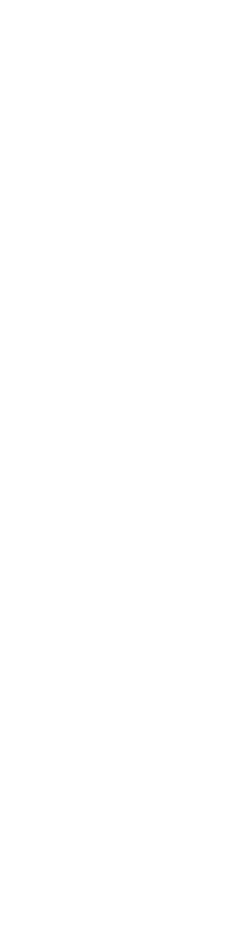
\includegraphics[width=3.5cm,angle=-90]{domaine1d}}
\caption{\label{Base_Covofi_domaine1d_fig}D\'efinition du domaine de calcul unidimensionnel
consid\'er\'e.}
\end{figure}


On s'int\'eresse \`a l'influence sur le respect du principe du maximum discret
de la pr\'ecision avec laquelle est v\'erifi\'ee sous forme discr\`ete la
relation~:
$$\forall i \in [1,N],\ \ \ \displaystyle\int_{\Omega_i}\dive\,(\rho\,\underline{u})\ d\Omega = 0$$
soit, ici~:
\begin{equation}
\label{Base_Covofi_ContinuiteDiscreteExemple}
-\,(\rho\ u)^n_{\,b_1}\,.\,S_{\,b_1}\,=\,(\rho\ u)^n_{\,12}\,.\,S_{\,12}\,
=\,(\rho\ u)^n_{\,23}\,.\,S_{\,23}\,=\,(\rho\ u)^n_{\,b_2}\,.\,S_{\,b_2}
\end{equation}

%-------------
\subsubsection*{Prise en compte de la contribution de
$\displaystyle\frac{\partial \rho}{\partial t}$ dans la matrice}
%-------------
\label{Base_Covofi_PpmaxAvecDrhoDt}
Le syst\`eme \`a r\'esoudre est alors, en omettant pour simplifier l'exposant $(\,n+1,k+1)$ :
\begin{equation}
\begin{array}{lllllllll}
&\displaystyle \rho_1^{\,n}\ \displaystyle\ \frac{|\Omega_1|}{\Delta
t}\,\delta f_1&&\ \ \ \ \ \ \ \    &-&(\rho\ u)^n_{\,b_1}\,.\,S_{\,b_1}\,\delta
f_1 &= &-(\rho\ u)^n_{\,b_1}\,.\,S_{\,b_1}\,f_{\,b_1}\\
&\displaystyle\rho_2^{\,n}\ \displaystyle\ \frac{|\Omega_2|}{\Delta
t}\,\delta f_2 &+&(\rho\ u)^n_{\,12}\,.\,S_{\,12}\,\delta f_2  &-&(\rho\
u)^n_{\,12}\,.\,S_{\,12}\,\delta f_1 &= &0\\
&\displaystyle\ \rho_3^{\,n} \displaystyle\ \frac{|\Omega_3|}{\Delta
t}\,\delta f_3 &+&(\rho\ u)^n_{\,23}\,.\,S_{\,23}\,\delta f_3 &-&(\rho\
u)^n_{\,23}\,.\,S_{\,23}\,\delta f_2 &= &0\\
\end{array}
\end{equation}
ce qui donne :
\begin{equation}
\left\{\begin{array}{lll}
&\delta f_1 =& \,f_{\,b_1}\displaystyle\ \frac{-(\rho\ u)^n_{\,b_1}\,.\,S_{\,b_1}}{\rho_1^{\,n}\ \displaystyle\ \frac{|\Omega_1|}{\Delta
t} - (\rho\ u)^n_{\,b_1}\,.\,S_{\,b_1}}\\
&\delta f_2 =&+ \,\delta f_1 \displaystyle\ \frac{(\rho\
u)^n_{\,12}\,.\,S_{\,12}}{\rho_2^{\,n}\ \displaystyle\ \frac{|\Omega_2|}{\Delta t} + (\rho\ u)^n_{\,12}\,.\,S_{\,12}}\\
&\delta f_3 =&+ \,\delta f_2 \displaystyle\ \frac{(\rho\
u)^n_{\,23}\,.\,S_{\,23}}{\rho_3^{\,n}\ \displaystyle\ \frac{|\Omega_3|}{\Delta
t} + (\rho\ u)^n_{\,23}\,.\,S_{\,23}}\\
\end{array}\right.
\end{equation}
d'o\`u :
\begin{equation}
\left\{\begin{array}{lll}
& \delta f_1 & <\ 1 \\
& \delta f_2 & <\ 1 \\
& \delta f_3 & <\ 1 \\
\end{array}\right.
\end{equation}
On obtient donc bien une solution qui v\'erifie le principe du maximum discret,
m\^eme pour des grands pas de temps $\Delta t$, et ce, quelle que soit la
pr\'ecision avec laquelle est v\'erifi\'ee, \`a l'\'etape de correction, la
forme discr\`ete (\ref{Base_Covofi_ContinuiteDiscreteExemple}) de la conservation de la
masse $\displaystyle\int_{\Omega_i}\dive\,(\rho\,\underline{u})\ d\Omega = 0$
dont on ne s'est pas servi ici.


%-------------
\subsubsection*{Sans la contribution de
$\displaystyle\frac{\partial \rho}{\partial t}$ dans la matrice}
%-------------


On obtient de m\^eme :
\begin{equation}
\begin{array}{lllllllll}
&\displaystyle \rho_1^{\,n}\ \displaystyle\ \frac{|\Omega_1|}{\Delta t}\,\delta f_1&+& (\rho\ u)^n_{\,12}\,.\,S_{\,12}\,\delta f_1& &\ \ \ \ \  &= &-(\rho\ u)^n_{\,b_1}\,.\,S_{\,b_1}\,f_{\,b_1}\\
&\displaystyle\rho_2^{\,n}\ \displaystyle\ \frac{|\Omega_2|}{\Delta
t}\,\delta f_2 &+&(\rho\ u)^n_{\,23}\,.\,S_{\,23}\,\delta f_2  &-&(\rho\
u)^n_{\,12}\,.\,S_{\,12}\,\delta f_1 &= &0\\
&\displaystyle\rho_3^{\,n}\ \displaystyle\ \frac{|\Omega_3|}{\Delta t}\,\delta
f_3 &-&(\rho\ u)^n_{\,23}\,.\,S_{\,23}\,\delta f_2     &+&(\rho\
u)^n_{\,b_2}\,.\,S_{\,b_2}\,\delta f_3 &= &0\\
\end{array}
\end{equation}

soit :

\begin{equation}
\left\{\begin{array}{lll}
&\delta f_1 =& \,f_{\,b_1}\displaystyle\ \frac{- ( \rho\ u)^n_{\,b_1}\,.\,S_{\,b_1}}{\rho_1^{\,n}\ \displaystyle\ \frac{|\Omega_1|}{\Delta
t} + (\rho\ u)^n_{\,12}\,.\,S_{\,12}}\\
&\delta f_2 =&\ \,\delta f_1 \displaystyle\ \frac{(\rho\
u)^n_{\,12}\,.\,S_{\,12}}{\rho_2^{\,n}\ \displaystyle\ \frac{|\Omega_2|}{\Delta t} + (\rho\ u)^n_{\,23}\,.\,S_{\,23}}\\
&\delta f_3 =&\ \,\delta f_2 \displaystyle\ \frac{(\rho\
u)^n_{\,23}\,.\,S_{\,23}}{\rho_3^{\,n}\ \displaystyle\ \frac{|\Omega_3|}{\Delta
t} + (\rho\ u)^n_{\,b_2}\,.\,S_{\,b_2}}\\
\end{array}\right.
\end{equation}
Ici, on constate que le respect du principe du maximum discret :\\
\begin{equation}
\left\{\begin{array}{lll}
&\delta f_1 &\leqslant \ 1 \\
&\delta f_2 &\leqslant \ 1 \\
&\delta f_3 &\leqslant \ 1 \\
\end{array}\right.
\end{equation}
est \'equivalent \`a la condition :
\begin{equation}
\left\{\begin{array}{lll}
- &( \rho\ u)^n_{\,b_1}\,.\,S_{\,b_1}&\leqslant \displaystyle\ \rho_1^{\,n}
\,\frac{|\Omega_1|}{\Delta t} + (\rho\ u)^n_{\,12}\,.\,S_{\,12}\\
&(\rho\ u)^n_{\,12}\,.\,S_{\,12}&\leqslant \displaystyle\ \rho_2^{\,n}
\frac{|\Omega_2|}{\Delta t} + (\rho\ u)^n_{\,23}\,.\,S_{\,23}\\
& (\rho\ u)^n_{\,23}\,.\,S_{\,23}&\leqslant \ \displaystyle\ \rho_3^{\,n}
\frac{|\Omega_3|}{\Delta t} + (\rho\ u)^n_{\,b_2}\,.\,S_{\,b_2}\\
\end{array}\right.
\end{equation}
Contrairement \`a la situation du paragraphe
\ref{Base_Covofi_PpmaxAvecDrhoDt}, on ne peut obtenir ici un r\'esultat qu'en
faisant intervenir l'\'egalit\'e (\ref{Base_Covofi_ContinuiteDiscreteExemple}), forme
discr\`ete de la conservation de la masse. On obtient bien alors, \`a partir du
syst\`eme pr\'ec\'edent~:
\begin{equation}
\left\{\begin{array}{lll}
&\delta f_1 &< \ 1 \\
&\delta f_2 &< \ 1 \\
&\delta f_3 &< \ 1 \\
\end{array}\right.
\end{equation}

Si l'on s'int\'eresse \`a la cellule $\Omega_1$ et que l'on
suppose $(\rho\ u)^n_{\,12}\,.\,S_{\,12}=-\,(\rho\
u)^n_{\,b_1}\,.\,S_{\,b_1}-\varepsilon (\rho\ u)^n_{\,12}\,.\,S_{\,12}$ (o\`u
$\varepsilon$ est la pr\'ecision locale relative pour l'\'equation de
conservation de la masse discr\`ete), on constate que l'on obtient $\delta\,f_1
> f_{b_1} = 1 $ (valeur non admissible) d\`es lors que~:
 $$\frac{1}{\varepsilon} < \frac{(\rho\
u)^n_{\,12}\,.\,S_{\,12}\Delta t}{\rho_1|\Omega_1|}$$
c'est-\`a-dire d\`es que
le nombre de CFL local $\displaystyle\frac{(\rho\
u)^n_{\,12}\,.\,S_{\,12}\Delta t}{\rho_1|\Omega_1|}$ exc\`ede l'inverse de la
pr\'ecision relative locale $\varepsilon$.

%=============
\subsection*{Conclusion}
%=============

Prendre en compte la contribution de
$\displaystyle\frac{\partial \rho}{\partial t}$ dans la matrice permet un meilleur respect du principe du maximum discret, lorsque la
pr\'ecision de $\displaystyle\int_{\Omega_i}\dive\,(\rho\,\underline{u})\
d\Omega = 0$ n'est pas exactement v\'erifi\'ee.
